\documentclass{beamer}
\usetheme{Antibes}
\usepackage{xcolor, colortbl}
\usepackage{algorithm}
\usepackage{algpseudocode}
\usepackage{textcomp}
\usepackage{listings}
\usepackage{hyperref}
\usepackage{alltt}
\usepackage{tikz}
\usepackage{framed}
\usepackage{marvosym}
\usepackage{wasysym}
\usepackage{marvosym}
\usepackage{crayola}
\usepackage{mathpartir}
\usepackage{tabularx}
\usepackage[belowskip=-15pt,aboveskip=0pt]{caption}
\usepackage[skins]{tcolorbox}
\usepackage{multicol}
\usetikzlibrary{positioning,shapes,arrows, arrows.meta, backgrounds, fit, shadows, automata}
\usetikzlibrary{decorations.markings, calc}
%\usepackage{wasysym}
%\usepackage{marvosym}
\setbeamertemplate{footline}[frame number]
%\usecolortheme{fly}
\usefonttheme{serif}

\title[Sujit]{Lexical Analysis \\
Programming Languages}
\author{Sujit Kumar Chakrabarti}
\institute{IIITB}
\date{}


\definecolor{lightblue}{rgb}{0.8,0.93,1.0} % color values Red, Green, Blue
\definecolor{darkblue}{rgb}{0.4,0.3,1.0} % color values Red, Green, Blue
\definecolor{Blue}{rgb}{0,0,1.0} % color values Red, Green, Blue
\definecolor{darkgreen}{rgb}{0,0.7,0.2} % color values Red, Green, Blue
\definecolor{Red}{rgb}{1,0,0} % color values Red, Green, Blue
\definecolor{Pink}{rgb}{0.7,0,0.2}
\definecolor{links}{HTML}{2A1B81}
\definecolor{mydarkgreen}{HTML}{126215}
\newcommand{\highlight}[1]{{\color{Red}(#1)}}

\newcommand{\myheader}[1]{
	{\color{darkblue}
		\begin{Large}
			\begin{center}
				{#1}
			\end{center}
		\end{Large}
	}
}
\newcommand{\myminorheader}[1]{
	{\color{BrickRed}
		\begin{Large}
			{\fontfamily{\sfdefault}\selectfont\textbf{#1}}
		\end{Large}
	}
}

%\tikzstyle{input} = [coordinate]
%\tikzstyle{output} = [coordinate]


\tikzstyle{bb}=[%
      rectangle, draw=black, thick, fill=OliveGreen!30, drop shadow, align=center,
      text ragged, minimum height=2em, minimum width=2em, inner sep=6pt
]

\tikzstyle{inv}=[%
      rectangle, draw=none,  align=center,
      text ragged, minimum height=2em, minimum width=2em, align=center, inner sep=6pt
]

\tikzstyle{db}=[%
      ellipse, draw=black, thick, fill=pink, drop shadow, align=center,
      text ragged, minimum height=2em, inner sep=6pt
]

\tikzstyle{jn}=[%
      inner sep=0cm, outer sep=0cm
]

\tikzstyle{io}=[%
      trapezium, trapezium left angle=60, trapezium right angle=120, draw=black, thick, fill=brown, drop shadow,
      text ragged, minimum height=2em, minimum width=2em, inner sep=6pt, align=center
]

\tikzstyle{glio}=[%
      trapezium, trapezium left angle=60, trapezium right angle=120, draw=red, line width = 1mm, fill=brown, drop shadow,
      text ragged, minimum height=2em, minimum width=2em, inner sep=6pt
]
\tikzstyle{gl}=[%
      rectangle, draw=red, line width = 1mm, fill=lightblue, drop shadow,
      text ragged, minimum height=2em, minimum width=2em, inner sep=6pt
]

\tikzstyle{en}=[%
      rectangle, draw=black, thick, fill=none,
      text ragged, minimum height=2em, minimum width=2em, inner sep=6pt
]

\tikzstyle{sh}=[%
      rectangle, draw=gray, thick, fill=none, color = gray,
      text ragged, minimum height=2em, minimum width=2em, inner sep=6pt
]


\lstdefinestyle{javacode}{
	language = Java,
	basicstyle = \ttfamily\scriptsize,
	stringstyle = \ttfamily,
	keywordstyle=\color{Blue}\bfseries,
	identifierstyle=\color{Pink},
	commentstyle=\color{darkgreen},
	frame=single,
	frameround=tttt,
%	numbers=left
	showstringspaces=false
}

\lstdefinestyle{camlcode}{
	language = Caml,
	basicstyle = \scriptsize\ttfamily,
	stringstyle = \color{red}\ttfamily,
	keywordstyle=\color{Blue}\bfseries,
	identifierstyle=\ttfamily,
	frame=single,
	frameround=tttt,
	numbers=none,
	showstringspaces=false,
	escapeinside={(*@}{@*)}
}

\lstdefinestyle{outputcode}{
	language = bash,
	backgroundcolor = \color{black},
	basicstyle = \tiny\ttfamily\color{white},
	stringstyle = \color{red}\ttfamily,
	keywordstyle=\color{white}\bfseries,
	identifierstyle=\ttfamily,
	frameround=tttt,
	numbers=none,
	showstringspaces=false,
	escapeinside={(*@}{@*)}
}

\newtcolorbox{myframe}[2][]{%
  enhanced,colback=white,colframe=black,coltitle=black,
  sharp corners,boxrule=0.4pt,
  fonttitle=\itshape,
  attach boxed title to top left={yshift=-0.3\baselineskip-0.4pt,xshift=2mm},
  boxed title style={tile,size=minimal,left=0.5mm,right=0.5mm,
    colback=white,before upper=\strut},
  title=#2,#1
}

\begin{document}
\maketitle

\section{Converting NFAs to DFAs}

% frame begin %%%%%%%%%%%%%%%%%%%%%%%%
\begin{frame}{NFA to DFA}
{Algorithm -- intuition}

\pause
\begin{itemize}
\item Start with the initial set (its $\epsilon$-closure).
\item For every symbol $a$ in $\Sigma$, compute the set of destination states (\textsc{move} followed by $\epsilon$-closure)
\item Discover new sets of states reachable by repeating this process.
\item Each new set of state is a distinct state in the resultant DFA.
\end{itemize}
\end{frame}
% frame end %%%%%%%%%%%%%%%%%%%%%%%%

% frame begin %%%%%%%%%%%%%%%%%%%%%%%%
\begin{frame}{NFA to DFA}
{Algorithm -- pseudocode}
\begin{footnotesize}
\begin{algorithmic}[0]
\Procedure{NFA2DFA}{$N$}
\pause
  \State $s_0' \gets$ \Call{$\epsilon$-closure}{$N.s_0$}
  \State add $s_0'$ to $D.states$
  \State \Call{unmark}{$s_0'$}
  \While{there is unmarked state $T$ in $D.states$}
    \State \Call{mark}{$T$}
    \ForAll{$a \in \sum$}
    	  \State $T' \gets$ \Call{move}{$T$, $a$}
      \State $\mathcal{U} \gets$ \Call{$\epsilon$-closure}{$T'$}
      \If{$\mathcal{U} \notin D.states$}
        \State add $\mathcal{U}$ to $D.states$
        \State \Call{unmark}{$\mathcal{U}$}
      \EndIf
    \EndFor
  \EndWhile
  \State \textbf{return} $D$
\EndProcedure

\end{algorithmic}
\end{footnotesize}
\end{frame}
% frame end %%%%%%%%%%%%%%%%%%%%%%%%


% frame begin %%%%%%%%%%%%%%%%%%%%%%%%
\begin{frame}{NFA to DFA}
{Algorithm -- Marking and Unmarking}

\begin{itemize}
\item An \emph{unmarked DFA-state} (a set of NFA-states) is one from which all outgoing transitions corresponding to each symbol in $\Sigma$ has not been explored.
\item For a \emph{marked DFA-state}, responses to all symbols of $\Sigma$ have been explored. 
\item A newly discovered DFA-state starts by being unmarked.
\item Could be implemented by maintaining a stack.
\item Algorithm terminates when the stack goes empty.
\end{itemize}
\end{frame}
% frame end %%%%%%%%%%%%%%%%%%%%%%%%

% frame begin %%%%%%%%%%%%%%%%%%%%%%%%
\begin{frame}{NFA to DFA}
\myminorheader{Example}

\textbf{NFA:}

\begin{center}
\resizebox{0.5\textwidth}{!}{%
\begin{tikzpicture}[auto,
    ->,
    -{Latex[length=3mm,width=2mm]}
  ]
    \node[initial, state]   (0)                       {$0$};
    \node[state]            (1)  [right = of 0]       {$1$};
    \node[state]            (2)  [above right = of 1] {$2$};
    \node[state]            (3)  [right = of 2]       {$3$};
    \node[state]            (4)  [below right = of 1] {$4$};
    \node[state]            (5)  [right = of 4]       {$5$};
    \node[state]            (6)  [below right = of 3] {$6$};
    \node[state]            (7)  [right = of 6]       {$7$};
    \node[state]            (8)  [right = of 7]       {$8$};
    \node[state]            (9)  [right = of 8]       {$9$};
    \node[state, accepting] (10) [right = of 9]       {$10$};
    
    \path (0) edge node {$\epsilon$} (1)
          (0) edge[bend right = 60] node {$\epsilon$} (7)
          (1) edge node {$\epsilon$} (2)
          (1) edge node {$\epsilon$} (4)
          (2) edge node {$a$} (3)
          (4) edge node {$b$} (5)
          (3) edge node {$\epsilon$} (6)
          (5) edge node {$\epsilon$} (6)
          (6) edge node {$\epsilon$} (7)
          (6.90) edge[bend right=90, min distance = 3 cm] node {$\epsilon$} (1.90)
          (7) edge node {$a$} (8)
          (8) edge node {$b$} (9)
          (9) edge node {$b$} (10)
          
          
    ;
    
  \end{tikzpicture}
}
\end{center}

\pause
\textbf{DFA:}
\begin{center}
\resizebox{0.4\textwidth}{!}{%
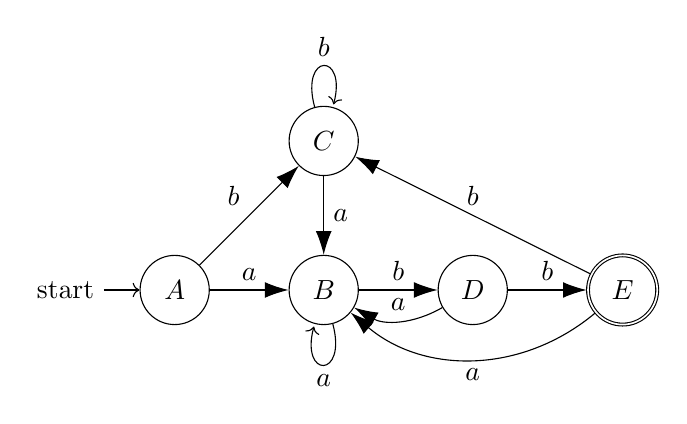
\begin{tikzpicture}[auto,
    ->,
    -{Latex[length=3mm,width=2mm]}
  ]
    \node[initial, state]   (A)                 {$A$};
    \node[state]            (B)  [right = of A] {$B$};
    \node[state]            (C)  [above = of B] {$C$};
    \node[state]            (D)  [right = of B] {$D$};
    \node[state, accepting] (E)  [right = of D] {$E$};
    
    \path (A) edge node {$a$} (B)
          (A) edge node {$b$} (C)
          (B) edge node {$b$} (D)
          (B) edge[loop below] node {$a$} (B)
          (C) edge node {$a$} (B)
          (C) edge[loop above] node {$b$} (C)
          (D) edge[bend left] node[above] {$a$} (B)
          (D) edge node {$b$} (E)
          (E) edge[bend left=40] node {$a$} (B)
          (E) edge node[above] {$b$} (C)
    ;
    
  \end{tikzpicture}
}
\end{center}
\end{frame}
% frame end %%%%%%%%%%%%%%%%%%%%%%%%

% frame begin %%%%%%%%%%%%%%%%%%%%%%%%
\begin{frame}{NFA to DFA}
\myminorheader{Example}

\textbf{NFA:}

\begin{center}
\resizebox{0.5\textwidth}{!}{%
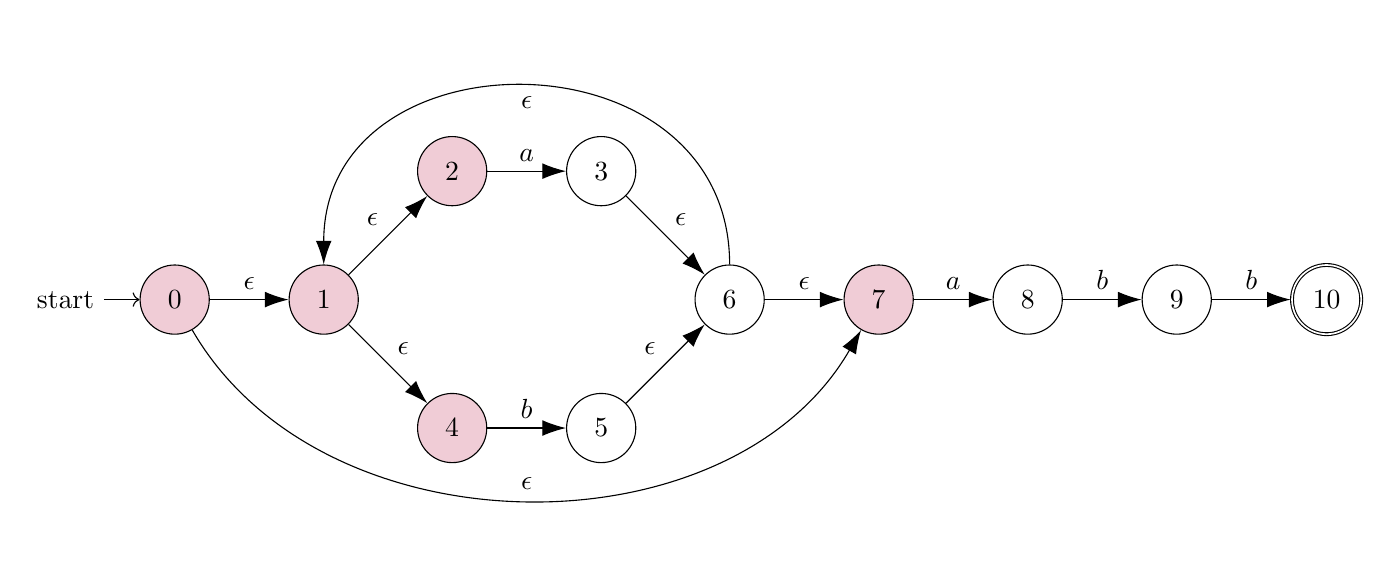
\begin{tikzpicture}[auto,
    ->,
    -{Latex[length=3mm,width=2mm]}
  ]
    \node[initial, state, fill=Pink!20]   (0)                       {$0$};
    \node[state, fill=Pink!20]            (1)  [right = of 0]       {$1$};
    \node[state, fill=Pink!20]            (2)  [above right = of 1] {$2$};
    \node[state]            (3)  [right = of 2]       {$3$};
    \node[state, fill=Pink!20]            (4)  [below right = of 1] {$4$};
    \node[state]            (5)  [right = of 4]       {$5$};
    \node[state]            (6)  [below right = of 3] {$6$};
    \node[state, fill=Pink!20]            (7)  [right = of 6]       {$7$};
    \node[state]            (8)  [right = of 7]       {$8$};
    \node[state]            (9)  [right = of 8]       {$9$};
    \node[state, accepting] (10) [right = of 9]       {$10$};
    
    \path (0) edge node {$\epsilon$} (1)
          (0) edge[bend right = 60] node {$\epsilon$} (7)
          (1) edge node {$\epsilon$} (2)
          (1) edge node {$\epsilon$} (4)
          (2) edge node {$a$} (3)
          (4) edge node {$b$} (5)
          (3) edge node {$\epsilon$} (6)
          (5) edge node {$\epsilon$} (6)
          (6) edge node {$\epsilon$} (7)
          (6.90) edge[bend right=90, min distance = 3 cm] node {$\epsilon$} (1.90)
          (7) edge node {$a$} (8)
          (8) edge node {$b$} (9)
          (9) edge node {$b$} (10)
          
          
    ;
    
  \end{tikzpicture}
}
\end{center}

\begin{tabular}{c @{\hspace{1cm}} c}
\begin{minipage}{0.3\textwidth}
\begin{tiny}
\begin{tabular}{|p{0.7\textwidth} | c | c |}
\hline
Subset & DFA & Marked \\
\hline
$\{0,1,2,4,7\}$       & $A$   & $\times$ \\
\hline
\end{tabular}
\end{tiny}
\end{minipage}
&
\begin{minipage}{0.7\textwidth}

\textbf{DFA:}
\begin{center}
\resizebox{0.6\textwidth}{!}{%
\begin{tikzpicture}[auto,
    ->,
    -{Latex[length=3mm,width=2mm]}
  ]
    \node[initial, state]   (A)                 {$A$};
    \node[state, draw=none]            (B)  [right = of A] {\ };
    \node[state, draw=none]            (C)  [above = of B] {\ };
    \node[state, draw=none]            (D)  [right = of B] {\ };
    \node[state, accepting, draw=none] (E)  [right = of D] {\ };
    
%    \path (A) edge node {$a$} (B)
%          (A) edge node {$b$} (C)
%          (B) edge node {$b$} (D)
%          (B) edge[loop below] node {$a$} (B)
%          (C) edge node {$a$} (B)
%          (C) edge[loop above] node {$b$} (C)
%          (D) edge[bend left] node[above] {$a$} (B)
%          (D) edge node {$b$} (E)
%          (E) edge[bend left=40] node {$a$} (B)
%          (E) edge node[above] {$b$} (C)
%    ;
    
  \end{tikzpicture}
}
\end{center}

\end{minipage}
\end{tabular}


\end{frame}
% frame end %%%%%%%%%%%%%%%%%%%%%%%%

% frame begin %%%%%%%%%%%%%%%%%%%%%%%%
\begin{frame}{NFA to DFA}
\myminorheader{Example}

\textbf{NFA:}

\begin{center}
\resizebox{0.5\textwidth}{!}{%
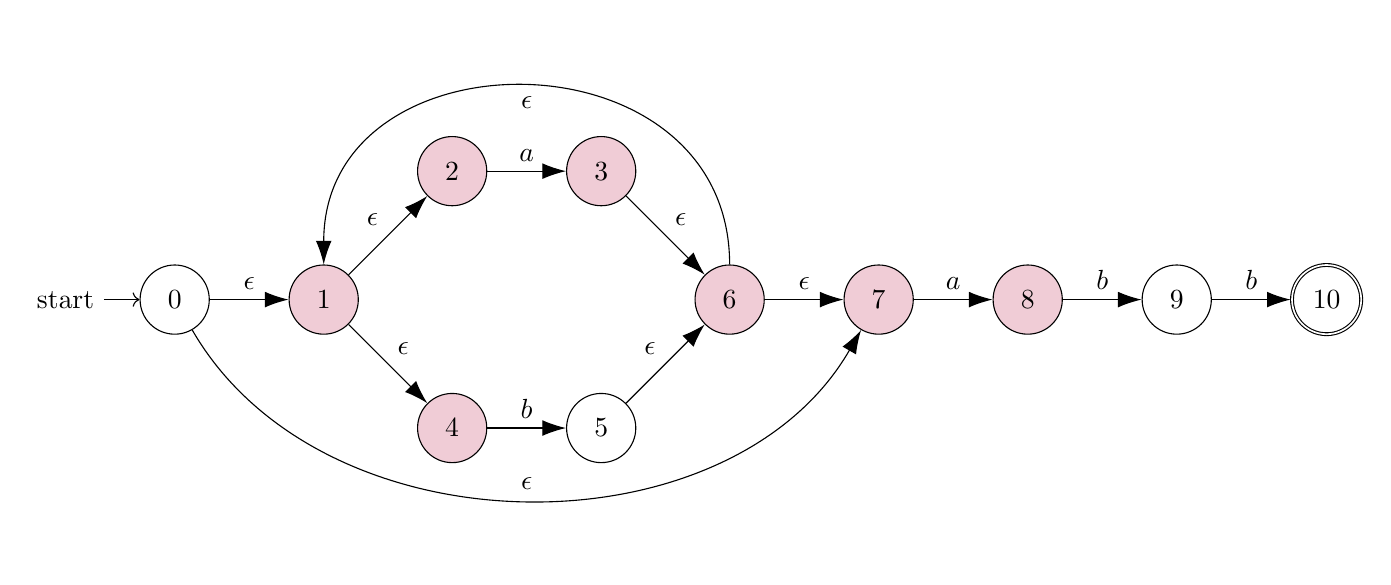
\begin{tikzpicture}[auto,
    ->,
    -{Latex[length=3mm,width=2mm]}
  ]
    \node[initial, state]   (0)                       {$0$};
    \node[state, fill=Pink!20]            (1)  [right = of 0]       {$1$};
    \node[state, fill=Pink!20]            (2)  [above right = of 1] {$2$};
    \node[state, fill=Pink!20]            (3)  [right = of 2]       {$3$};
    \node[state, fill=Pink!20]            (4)  [below right = of 1] {$4$};
    \node[state]            (5)  [right = of 4]       {$5$};
    \node[state, fill=Pink!20]            (6)  [below right = of 3] {$6$};
    \node[state, fill=Pink!20]            (7)  [right = of 6]       {$7$};
    \node[state, fill=Pink!20]            (8)  [right = of 7]       {$8$};
    \node[state]            (9)  [right = of 8]       {$9$};
    \node[state, accepting] (10) [right = of 9]       {$10$};
    
    \path (0) edge node {$\epsilon$} (1)
          (0) edge[bend right = 60] node {$\epsilon$} (7)
          (1) edge node {$\epsilon$} (2)
          (1) edge node {$\epsilon$} (4)
          (2) edge node {$a$} (3)
          (4) edge node {$b$} (5)
          (3) edge node {$\epsilon$} (6)
          (5) edge node {$\epsilon$} (6)
          (6) edge node {$\epsilon$} (7)
          (6.90) edge[bend right=90, min distance = 3 cm] node {$\epsilon$} (1.90)
          (7) edge node {$a$} (8)
          (8) edge node {$b$} (9)
          (9) edge node {$b$} (10)
          
          
    ;
    
  \end{tikzpicture}
}
  
{\scriptsize$DTrans(\{0,1,2,4,7\}, a) = \{1,2,3,4,6,7,8\}$}
\end{center}

\begin{tabular}{c @{\hspace{1cm}} c}
\begin{minipage}{0.3\textwidth}
\begin{tiny}
\begin{tabular}{|p{0.7\textwidth} | c | c |}
\hline
Subset & DFA & Marked \\
\hline
$\{0,1,2,4,7\}$       & $A$   & $\times$ \\
\hline
$\{1,2,3,4,6,7,8\}$       & $B$   & $\times$ \\
\hline
\end{tabular}
\end{tiny}
\end{minipage}
&
\begin{minipage}{0.7\textwidth}

\textbf{DFA:}
\begin{center}
\resizebox{0.6\textwidth}{!}{%
\begin{tikzpicture}[auto,
    ->,
    -{Latex[length=3mm,width=2mm]}
  ]
    \node[initial, state]   (A)                 {$A$};
    \node[state, draw=Black]            (B)  [right = of A] {$B$};
    \node[state, draw=none]            (C)  [above = of B] {\ };
    \node[state, draw=none]            (D)  [right = of B] {\ };
    \node[state, accepting, draw=none] (E)  [right = of D] {\ };
    
    \path (A) edge node {$a$} (B)
%          (A) edge node {$b$} (C)
%          (B) edge node {$b$} (D)
%          (B) edge[loop below] node {$a$} (B)
%          (C) edge node {$a$} (B)
%          (C) edge[loop above] node {$b$} (C)
%          (D) edge[bend left] node[above] {$a$} (B)
%          (D) edge node {$b$} (E)
%          (E) edge[bend left=40] node {$a$} (B)
%          (E) edge node[above] {$b$} (C)
    ;
    
  \end{tikzpicture}
}
\end{center}

\end{minipage}
\end{tabular}

\end{frame}
% frame end %%%%%%%%%%%%%%%%%%%%%%%%

% frame begin %%%%%%%%%%%%%%%%%%%%%%%%
\begin{frame}{NFA to DFA}
\myminorheader{Example}

\textbf{NFA:}

\begin{center}
\resizebox{0.5\textwidth}{!}{%
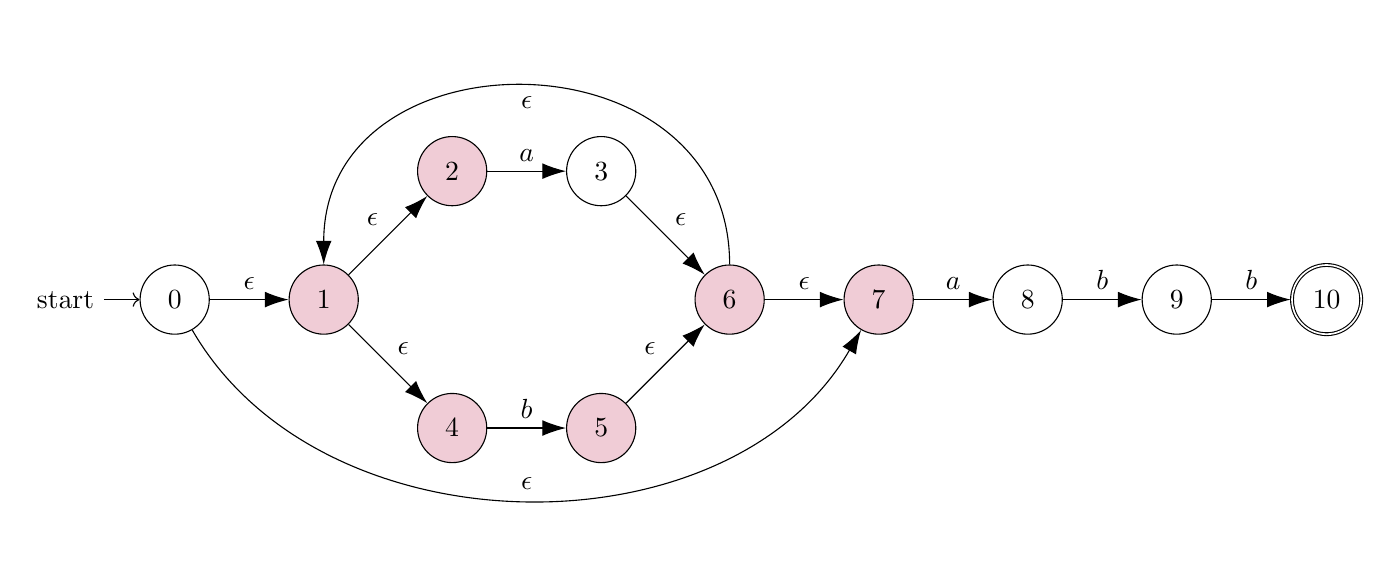
\begin{tikzpicture}[auto,
    ->,
    -{Latex[length=3mm,width=2mm]}
  ]
    \node[initial, state]   (0)                       {$0$};
    \node[state, fill=Pink!20]            (1)  [right = of 0]       {$1$};
    \node[state, fill=Pink!20]            (2)  [above right = of 1] {$2$};
    \node[state]            (3)  [right = of 2]       {$3$};
    \node[state, fill=Pink!20]            (4)  [below right = of 1] {$4$};
    \node[state, fill=Pink!20]            (5)  [right = of 4]       {$5$};
    \node[state, fill=Pink!20]            (6)  [below right = of 3] {$6$};
    \node[state, fill=Pink!20]            (7)  [right = of 6]       {$7$};
    \node[state]            (8)  [right = of 7]       {$8$};
    \node[state]            (9)  [right = of 8]       {$9$};
    \node[state, accepting] (10) [right = of 9]       {$10$};
    
    \path (0) edge node {$\epsilon$} (1)
          (0) edge[bend right = 60] node {$\epsilon$} (7)
          (1) edge node {$\epsilon$} (2)
          (1) edge node {$\epsilon$} (4)
          (2) edge node {$a$} (3)
          (4) edge node {$b$} (5)
          (3) edge node {$\epsilon$} (6)
          (5) edge node {$\epsilon$} (6)
          (6) edge node {$\epsilon$} (7)
          (6.90) edge[bend right=90, min distance = 3 cm] node {$\epsilon$} (1.90)
          (7) edge node {$a$} (8)
          (8) edge node {$b$} (9)
          (9) edge node {$b$} (10)
          
          
    ;
    
  \end{tikzpicture}
}

{\scriptsize$DTrans(\{0,1,2,4,7\}, b) = \{1,2,4,5,6,7\}$}
\end{center}
\begin{tabular}{c @{\hspace{1cm}} c}
\begin{minipage}{0.3\textwidth}
\begin{tiny}
\begin{tabular}{|p{0.7\textwidth} | c | c |}
\hline
Subset & DFA & Marked \\
\hline
$\{0,1,2,4,7\}$       & $A$   & $\checkmark$ \\
\hline
$\{1,2,3,4,6,7,8\}$       & $B$   & $\times$ \\
\hline
$\{1,2,4,5,6,7\}$       & $C$   & $\times$ \\
\hline
\end{tabular}
\end{tiny}
\end{minipage}
&
\begin{minipage}{0.7\textwidth}

\textbf{DFA:}
\begin{center}
\resizebox{0.6\textwidth}{!}{%
\begin{tikzpicture}[auto,
    ->,
    -{Latex[length=3mm,width=2mm]}
  ]
    \node[initial, state]   (A)                 {$A$};
    \node[state, draw=Black]            (B)  [right = of A] {$B$};
    \node[state, draw=Black]            (C)  [above = of B] {$C$};
    \node[state, draw=none]            (D)  [right = of B] {\ };
    \node[state, accepting, draw=none] (E)  [right = of D] {\ };
    
    \path (A) edge node {$a$} (B)
          (A) edge node {$b$} (C)
%          (B) edge node {$b$} (D)
%          (B) edge[loop below] node {$a$} (B)
%          (C) edge node {$a$} (B)
%          (C) edge[loop above] node {$b$} (C)
%          (D) edge[bend left] node[above] {$a$} (B)
%          (D) edge node {$b$} (E)
%          (E) edge[bend left=40] node {$a$} (B)
%          (E) edge node[above] {$b$} (C)
    ;
    
  \end{tikzpicture}
}
\end{center}

\end{minipage}
\end{tabular}

\end{frame}
% frame end %%%%%%%%%%%%%%%%%%%%%%%%


% frame begin %%%%%%%%%%%%%%%%%%%%%%%%
\begin{frame}{NFA to DFA}
\myminorheader{Example}

\textbf{NFA:}

\begin{center}
\resizebox{0.5\textwidth}{!}{%
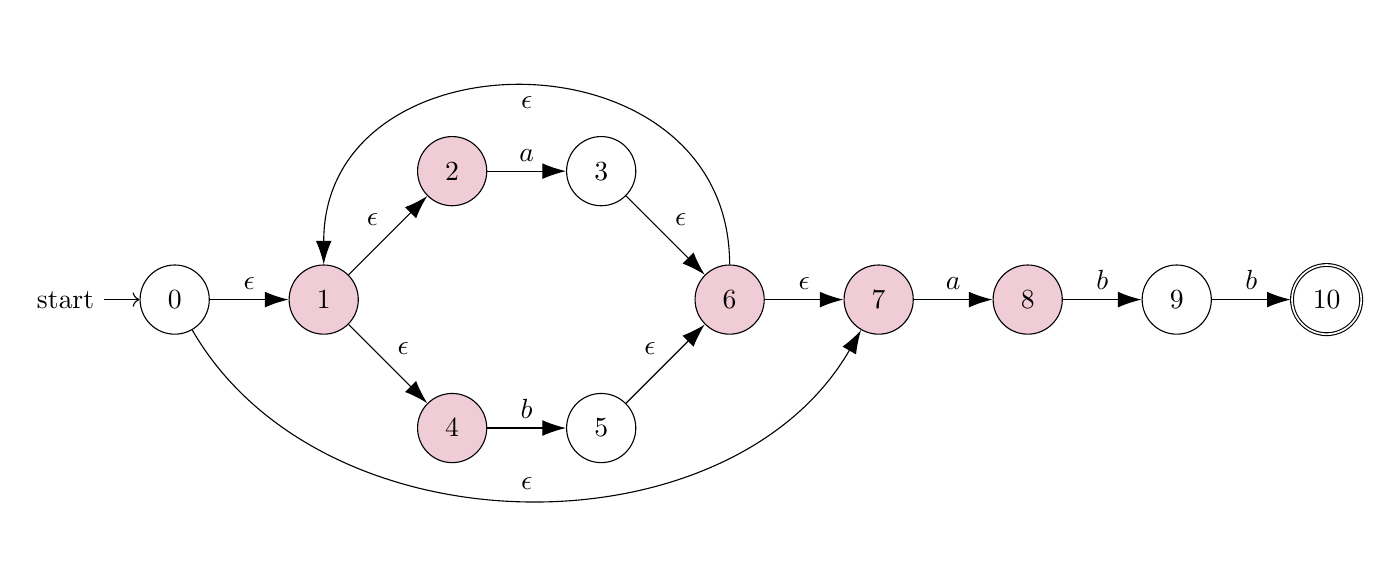
\begin{tikzpicture}[auto,
    ->,
    -{Latex[length=3mm,width=2mm]}
  ]
    \node[initial, state]   (0)                       {$0$};
    \node[state, fill=Pink!20]            (1)  [right = of 0]       {$1$};
    \node[state, fill=Pink!20]            (2)  [above right = of 1] {$2$};
    \node[state]            (3)  [right = of 2]       {$3$};
    \node[state, fill=Pink!20]            (4)  [below right = of 1] {$4$};
    \node[state]            (5)  [right = of 4]       {$5$};
    \node[state, fill=Pink!20]            (6)  [below right = of 3] {$6$};
    \node[state, fill=Pink!20]            (7)  [right = of 6]       {$7$};
    \node[state, fill=Pink!20]            (8)  [right = of 7]       {$8$};
    \node[state]            (9)  [right = of 8]       {$9$};
    \node[state, accepting] (10) [right = of 9]       {$10$};
    
    \path (0) edge node {$\epsilon$} (1)
          (0) edge[bend right = 60] node {$\epsilon$} (7)
          (1) edge node {$\epsilon$} (2)
          (1) edge node {$\epsilon$} (4)
          (2) edge node {$a$} (3)
          (4) edge node {$b$} (5)
          (3) edge node {$\epsilon$} (6)
          (5) edge node {$\epsilon$} (6)
          (6) edge node {$\epsilon$} (7)
          (6.90) edge[bend right=90, min distance = 3 cm] node {$\epsilon$} (1.90)
          (7) edge node {$a$} (8)
          (8) edge node {$b$} (9)
          (9) edge node {$b$} (10)
          
          
    ;
    
  \end{tikzpicture}
}

{\scriptsize$DTrans(\{1,2,3,4,6,7,8\}, a) = \{1,2,3,4,6,7,8\}$}
\end{center}

\begin{tabular}{c @{\hspace{1cm}} c}
\begin{minipage}{0.3\textwidth}
\begin{tiny}
\begin{tabular}{|p{0.7\textwidth} | c | c |}
\hline
Subset & DFA & Marked \\
\hline
$\{0,1,2,4,7\}$       & $A$   & $\checkmark$ \\
\hline
$\{1,2,3,4,6,7,8\}$       & $B$   & $\times$ \\
\hline
$\{1,2,4,5,6,7\}$       & $C$   & $\times$ \\
\hline
\end{tabular}
\end{tiny}
\end{minipage}
&
\begin{minipage}{0.7\textwidth}

\textbf{DFA:}
\begin{center}
\resizebox{0.6\textwidth}{!}{%
\begin{tikzpicture}[auto,
    ->,
    -{Latex[length=3mm,width=2mm]}
  ]
    \node[initial, state]   (A)                 {$A$};
    \node[state, draw=Black]            (B)  [right = of A] {$B$};
    \node[state, draw=Black]            (C)  [above = of B] {$C$};
    \node[state, draw=none]            (D)  [right = of B] {\ };
    \node[state, accepting, draw=none] (E)  [right = of D] {\ };
    
    \path (A) edge node {$a$} (B)
          (A) edge node {$b$} (C)
%          (B) edge node {$b$} (D)
          (B) edge[loop below] node {$a$} (B)
%          (C) edge node {$a$} (B)
%          (C) edge[loop above] node {$b$} (C)
%          (D) edge[bend left] node[above] {$a$} (B)
%          (D) edge node {$b$} (E)
%          (E) edge[bend left=40] node {$a$} (B)
%          (E) edge node[above] {$b$} (C)
    ;
    
  \end{tikzpicture}
}
\end{center}

\end{minipage}
\end{tabular}

\end{frame}
% frame end %%%%%%%%%%%%%%%%%%%%%%%%

% frame begin %%%%%%%%%%%%%%%%%%%%%%%%
\begin{frame}{NFA to DFA}
\myminorheader{Example}

\textbf{NFA:}

\begin{center}
\resizebox{0.5\textwidth}{!}{%
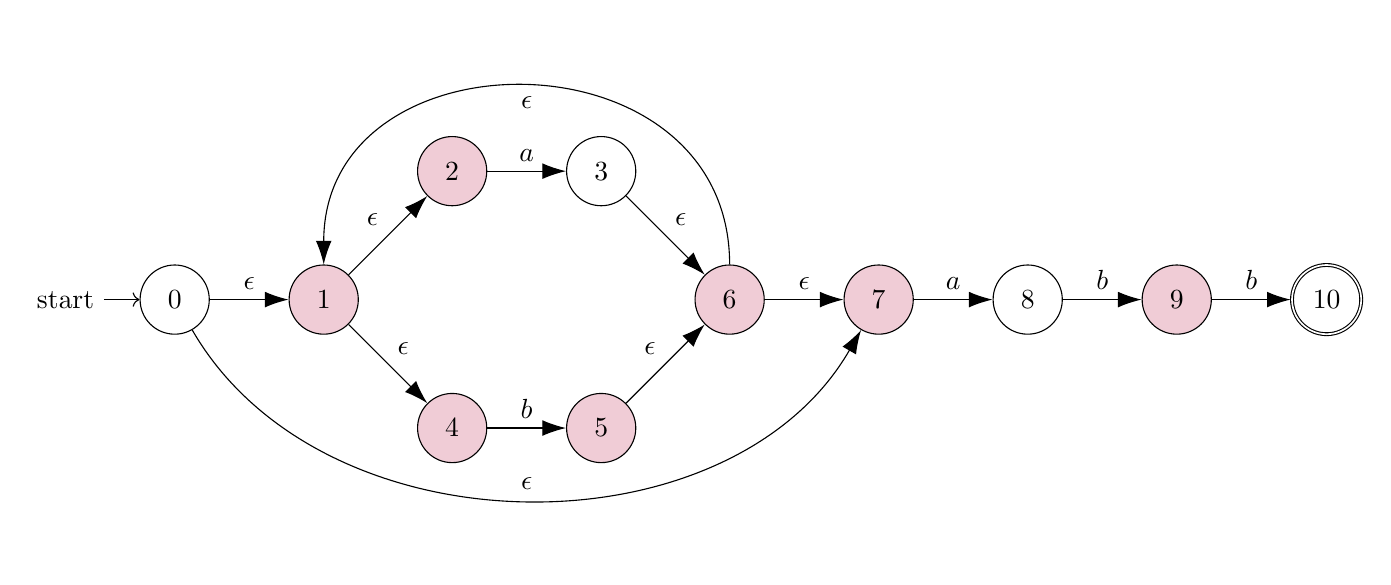
\begin{tikzpicture}[auto,
    ->,
    -{Latex[length=3mm,width=2mm]}
  ]
    \node[initial, state]   (0)                       {$0$};
    \node[state, fill=Pink!20]            (1)  [right = of 0]       {$1$};
    \node[state, fill=Pink!20]            (2)  [above right = of 1] {$2$};
    \node[state]            (3)  [right = of 2]       {$3$};
    \node[state, fill=Pink!20]            (4)  [below right = of 1] {$4$};
    \node[state, fill=Pink!20]            (5)  [right = of 4]       {$5$};
    \node[state, fill=Pink!20]            (6)  [below right = of 3] {$6$};
    \node[state, fill=Pink!20]            (7)  [right = of 6]       {$7$};
    \node[state]            (8)  [right = of 7]       {$8$};
    \node[state, fill=Pink!20]            (9)  [right = of 8]       {$9$};
    \node[state, accepting] (10) [right = of 9]       {$10$};
    
    \path (0) edge node {$\epsilon$} (1)
          (0) edge[bend right = 60] node {$\epsilon$} (7)
          (1) edge node {$\epsilon$} (2)
          (1) edge node {$\epsilon$} (4)
          (2) edge node {$a$} (3)
          (4) edge node {$b$} (5)
          (3) edge node {$\epsilon$} (6)
          (5) edge node {$\epsilon$} (6)
          (6) edge node {$\epsilon$} (7)
          (6.90) edge[bend right=90, min distance = 3 cm] node {$\epsilon$} (1.90)
          (7) edge node {$a$} (8)
          (8) edge node {$b$} (9)
          (9) edge node {$b$} (10)
          
          
    ;
    
  \end{tikzpicture}
}

{\scriptsize$DTrans(\{1,2,3,4,6,7,8\}, b) = \{1,2,4,5,6,7,9\}$}
\end{center}

\begin{tabular}{c @{\hspace{1cm}} c}
\begin{minipage}{0.3\textwidth}
\begin{tiny}
\begin{tabular}{|p{0.7\textwidth} | c | c |}
\hline
Subset & DFA & Marked \\
\hline
$\{0,1,2,4,7\}$       & $A$   & $\checkmark$ \\
\hline
$\{1,2,3,4,6,7,8\}$       & $B$   & $\checkmark$ \\
\hline
$\{1,2,4,5,6,7\}$       & $C$   & $\times$ \\
\hline
$\{1,2,4,5,6,7,9\}$       & $D$   & $\times$ \\
\hline
\end{tabular}
\end{tiny}
\end{minipage}
&
\begin{minipage}{0.7\textwidth}

\textbf{DFA:}
\begin{center}
\resizebox{0.6\textwidth}{!}{%
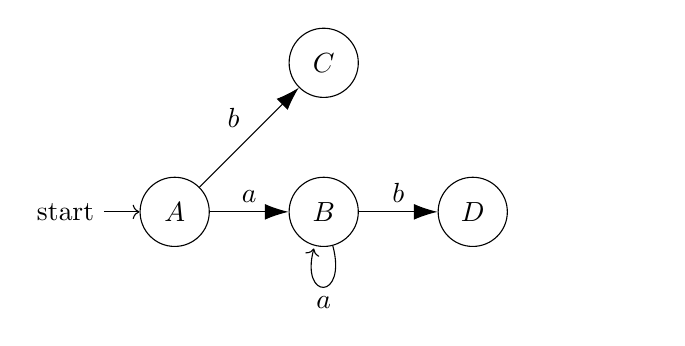
\begin{tikzpicture}[auto,
    ->,
    -{Latex[length=3mm,width=2mm]}
  ]
    \node[initial, state]   (A)                 {$A$};
    \node[state, draw=Black]            (B)  [right = of A] {$B$};
    \node[state, draw=Black]            (C)  [above = of B] {$C$};
    \node[state, draw=Black]            (D)  [right = of B] {$D$};
    \node[state, accepting, draw=none] (E)  [right = of D] {\ };
    
    \path (A) edge node {$a$} (B)
          (A) edge node {$b$} (C)
          (B) edge node {$b$} (D)
          (B) edge[loop below] node {$a$} (B)
%          (C) edge node {$a$} (B)
%          (C) edge[loop above] node {$b$} (C)
%          (D) edge[bend left] node[above] {$a$} (B)
%          (D) edge node {$b$} (E)
%          (E) edge[bend left=40] node {$a$} (B)
%          (E) edge node[above] {$b$} (C)
    ;
    
  \end{tikzpicture}
}
\end{center}

\end{minipage}
\end{tabular}

\end{frame}
% frame end %%%%%%%%%%%%%%%%%%%%%%%%

% frame begin %%%%%%%%%%%%%%%%%%%%%%%%
\begin{frame}{NFA to DFA}
\myminorheader{Example}

\textbf{NFA:}

\begin{center}
\resizebox{0.5\textwidth}{!}{%
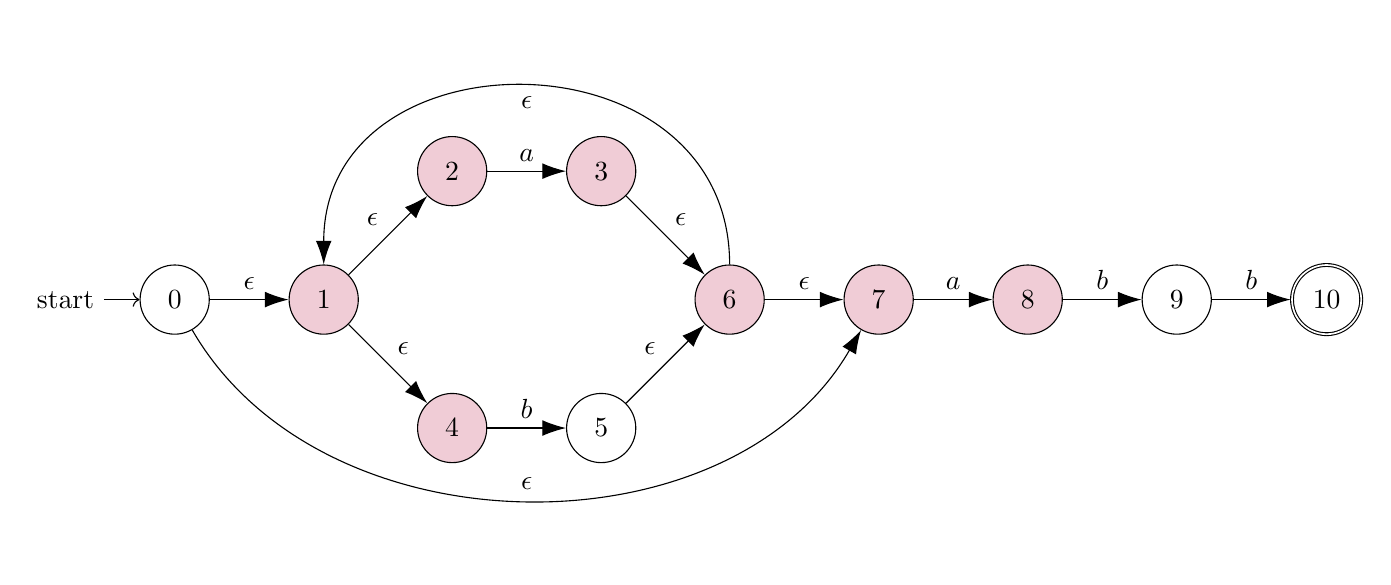
\begin{tikzpicture}[auto,
    ->,
    -{Latex[length=3mm,width=2mm]}
  ]
    \node[initial, state]   (0)                       {$0$};
    \node[state, fill=Pink!20]            (1)  [right = of 0]       {$1$};
    \node[state, fill=Pink!20]            (2)  [above right = of 1] {$2$};
    \node[state, fill=Pink!20]            (3)  [right = of 2]       {$3$};
    \node[state, fill=Pink!20]            (4)  [below right = of 1] {$4$};
    \node[state]            (5)  [right = of 4]       {$5$};
    \node[state, fill=Pink!20]            (6)  [below right = of 3] {$6$};
    \node[state, fill=Pink!20]            (7)  [right = of 6]       {$7$};
    \node[state, fill=Pink!20]            (8)  [right = of 7]       {$8$};
    \node[state]            (9)  [right = of 8]       {$9$};
    \node[state, accepting] (10) [right = of 9]       {$10$};
    
    \path (0) edge node {$\epsilon$} (1)
          (0) edge[bend right = 60] node {$\epsilon$} (7)
          (1) edge node {$\epsilon$} (2)
          (1) edge node {$\epsilon$} (4)
          (2) edge node {$a$} (3)
          (4) edge node {$b$} (5)
          (3) edge node {$\epsilon$} (6)
          (5) edge node {$\epsilon$} (6)
          (6) edge node {$\epsilon$} (7)
          (6.90) edge[bend right=90, min distance = 3 cm] node {$\epsilon$} (1.90)
          (7) edge node {$a$} (8)
          (8) edge node {$b$} (9)
          (9) edge node {$b$} (10)
          
          
    ;
    
  \end{tikzpicture}
}

{\scriptsize$DTrans(\{1,2,4,5,6,7\}, a) = \{1,2,3,4,6,7,8\}$}
\end{center}

\begin{tabular}{c @{\hspace{1cm}} c}
\begin{minipage}{0.3\textwidth}
\begin{tiny}
\begin{tabular}{|p{0.7\textwidth} | c | c |}
\hline
Subset & DFA & Marked \\
\hline
$\{0,1,2,4,7\}$       & $A$   & $\checkmark$ \\
\hline
$\{1,2,3,4,6,7,8\}$       & $B$   & $\checkmark$ \\
\hline
$\{1,2,4,5,6,7\}$       & $C$   & $\times$ \\
\hline
$\{1,2,4,5,6,7,9\}$       & $D$   & $\times$ \\
\hline
\end{tabular}
\end{tiny}
\end{minipage}
&
\begin{minipage}{0.7\textwidth}

\textbf{DFA:}
\begin{center}
\resizebox{0.6\textwidth}{!}{%
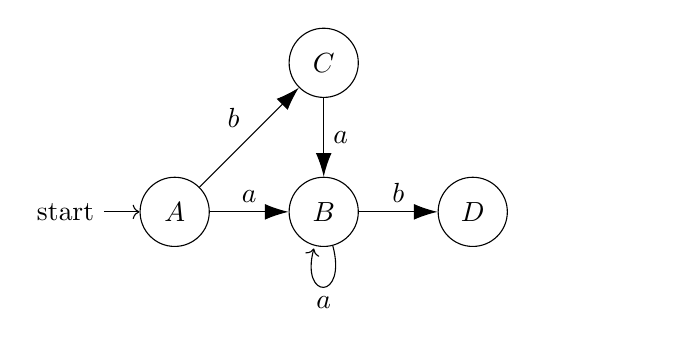
\begin{tikzpicture}[auto,
    ->,
    -{Latex[length=3mm,width=2mm]}
  ]
    \node[initial, state]   (A)                 {$A$};
    \node[state, draw=Black]            (B)  [right = of A] {$B$};
    \node[state, draw=Black]            (C)  [above = of B] {$C$};
    \node[state, draw=Black]            (D)  [right = of B] {$D$};
    \node[state, accepting, draw=none] (E)  [right = of D] {\ };
    
    \path (A) edge node {$a$} (B)
          (A) edge node {$b$} (C)
          (B) edge node {$b$} (D)
          (B) edge[loop below] node {$a$} (B)
          (C) edge node {$a$} (B)
%          (C) edge[loop above] node {$b$} (C)
%          (D) edge[bend left] node[above] {$a$} (B)
%          (D) edge node {$b$} (E)
%          (E) edge[bend left=40] node {$a$} (B)
%          (E) edge node[above] {$b$} (C)
    ;
    
  \end{tikzpicture}
}
\end{center}

\end{minipage}
\end{tabular}

\end{frame}
% frame end %%%%%%%%%%%%%%%%%%%%%%%%

% frame begin %%%%%%%%%%%%%%%%%%%%%%%%
\begin{frame}{NFA to DFA}
\myminorheader{Example}

\textbf{NFA:}

\begin{center}
\resizebox{0.5\textwidth}{!}{%
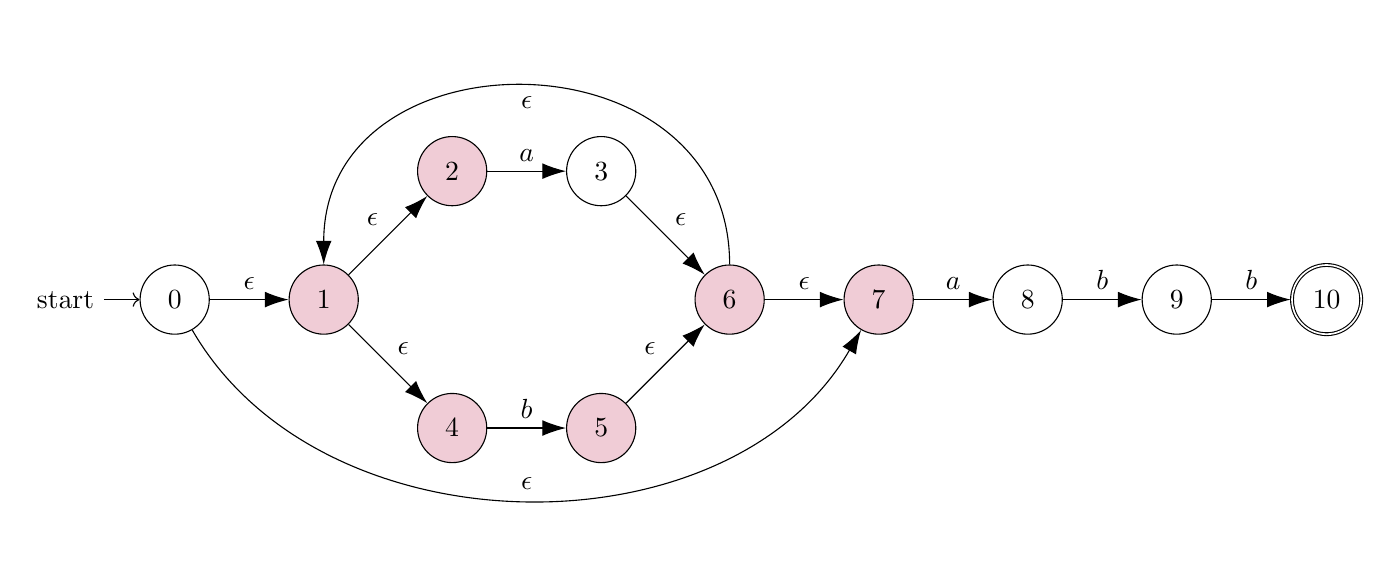
\begin{tikzpicture}[auto,
    ->,
    -{Latex[length=3mm,width=2mm]}
  ]
    \node[initial, state]   (0)                       {$0$};
    \node[state, fill=Pink!20]            (1)  [right = of 0]       {$1$};
    \node[state, fill=Pink!20]            (2)  [above right = of 1] {$2$};
    \node[state]            (3)  [right = of 2]       {$3$};
    \node[state, fill=Pink!20]            (4)  [below right = of 1] {$4$};
    \node[state, fill=Pink!20]            (5)  [right = of 4]       {$5$};
    \node[state, fill=Pink!20]            (6)  [below right = of 3] {$6$};
    \node[state, fill=Pink!20]            (7)  [right = of 6]       {$7$};
    \node[state]            (8)  [right = of 7]       {$8$};
    \node[state]            (9)  [right = of 8]       {$9$};
    \node[state, accepting] (10) [right = of 9]       {$10$};
    
    \path (0) edge node {$\epsilon$} (1)
          (0) edge[bend right = 60] node {$\epsilon$} (7)
          (1) edge node {$\epsilon$} (2)
          (1) edge node {$\epsilon$} (4)
          (2) edge node {$a$} (3)
          (4) edge node {$b$} (5)
          (3) edge node {$\epsilon$} (6)
          (5) edge node {$\epsilon$} (6)
          (6) edge node {$\epsilon$} (7)
          (6.90) edge[bend right=90, min distance = 3 cm] node {$\epsilon$} (1.90)
          (7) edge node {$a$} (8)
          (8) edge node {$b$} (9)
          (9) edge node {$b$} (10)
          
          
    ;
    
  \end{tikzpicture}
}

{\scriptsize$DTrans(\{1,2,4,5,6,7\}, b) = \{1,2,4,5,6,7\}$}
\end{center}

\begin{tabular}{c @{\hspace{1cm}} c}
\begin{minipage}{0.3\textwidth}
\begin{tiny}
\begin{tabular}{|p{0.7\textwidth} | c | c |}
\hline
Subset & DFA & Marked \\
\hline
$\{0,1,2,4,7\}$       & $A$   & $\checkmark$ \\
\hline
$\{1,2,3,4,6,7,8\}$       & $B$   & $\checkmark$ \\
\hline
$\{1,2,4,5,6,7\}$       & $C$   & $\checkmark$ \\
\hline
$\{1,2,4,5,6,7,9\}$       & $D$   & $\times$ \\
\hline
\end{tabular}
\end{tiny}
\end{minipage}
&
\begin{minipage}{0.7\textwidth}

\textbf{DFA:}
\begin{center}
\resizebox{0.6\textwidth}{!}{%
\begin{tikzpicture}[auto,
    ->,
    -{Latex[length=3mm,width=2mm]}
  ]
    \node[initial, state]   (A)                 {$A$};
    \node[state, draw=Black]            (B)  [right = of A] {$B$};
    \node[state, draw=Black]            (C)  [above = of B] {$C$};
    \node[state, draw=Black]            (D)  [right = of B] {$D$};
    \node[state, accepting, draw=none] (E)  [right = of D] {\ };
    
    \path (A) edge node {$a$} (B)
          (A) edge node {$b$} (C)
          (B) edge node {$b$} (D)
          (B) edge[loop below] node {$a$} (B)
          (C) edge node {$a$} (B)
          (C) edge[loop above] node {$b$} (C)
%          (D) edge[bend left] node[above] {$a$} (B)
%          (D) edge node {$b$} (E)
%          (E) edge[bend left=40] node {$a$} (B)
%          (E) edge node[above] {$b$} (C)
    ;
    
  \end{tikzpicture}
}
\end{center}

\end{minipage}
\end{tabular}

\end{frame}
% frame end %%%%%%%%%%%%%%%%%%%%%%%%

% frame begin %%%%%%%%%%%%%%%%%%%%%%%%
\begin{frame}{NFA to DFA}
\myminorheader{Example}

\textbf{NFA:}

\begin{center}
\resizebox{0.5\textwidth}{!}{%
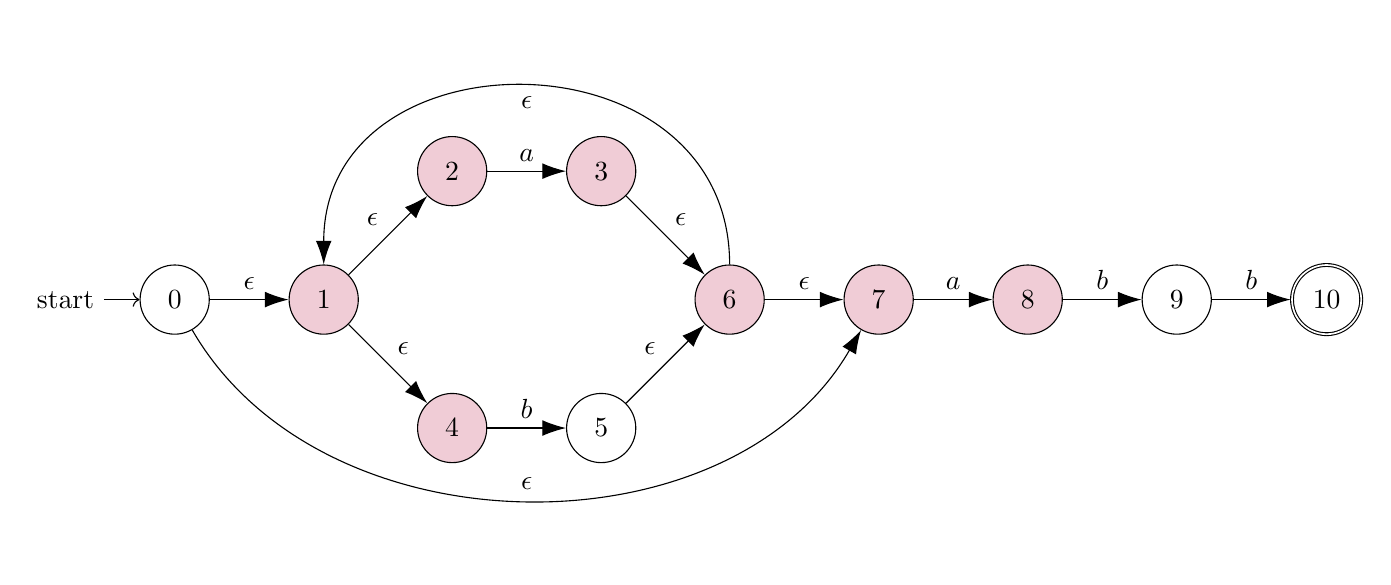
\begin{tikzpicture}[auto,
    ->,
    -{Latex[length=3mm,width=2mm]}
  ]
    \node[initial, state]   (0)                       {$0$};
    \node[state, fill=Pink!20]            (1)  [right = of 0]       {$1$};
    \node[state, fill=Pink!20]            (2)  [above right = of 1] {$2$};
    \node[state, fill=Pink!20]            (3)  [right = of 2]       {$3$};
    \node[state, fill=Pink!20]            (4)  [below right = of 1] {$4$};
    \node[state]            (5)  [right = of 4]       {$5$};
    \node[state, fill=Pink!20]            (6)  [below right = of 3] {$6$};
    \node[state, fill=Pink!20]            (7)  [right = of 6]       {$7$};
    \node[state, fill=Pink!20]            (8)  [right = of 7]       {$8$};
    \node[state]            (9)  [right = of 8]       {$9$};
    \node[state, accepting] (10) [right = of 9]       {$10$};
    
    \path (0) edge node {$\epsilon$} (1)
          (0) edge[bend right = 60] node {$\epsilon$} (7)
          (1) edge node {$\epsilon$} (2)
          (1) edge node {$\epsilon$} (4)
          (2) edge node {$a$} (3)
          (4) edge node {$b$} (5)
          (3) edge node {$\epsilon$} (6)
          (5) edge node {$\epsilon$} (6)
          (6) edge node {$\epsilon$} (7)
          (6.90) edge[bend right=90, min distance = 3 cm] node {$\epsilon$} (1.90)
          (7) edge node {$a$} (8)
          (8) edge node {$b$} (9)
          (9) edge node {$b$} (10)
          
          
    ;
    
  \end{tikzpicture}
}

{\scriptsize$DTrans(\{1,2,4,5,6,7,9\}, a) = \{1,2,3,4,6,7,8\}$}
\end{center}

\begin{tabular}{c @{\hspace{1cm}} c}
\begin{minipage}{0.3\textwidth}
\begin{tiny}
\begin{tabular}{|p{0.7\textwidth} | c | c |}
\hline
Subset & DFA & Marked \\
\hline
$\{0,1,2,4,7\}$       & $A$   & $\checkmark$ \\
\hline
$\{1,2,3,4,6,7,8\}$       & $B$   & $\checkmark$ \\
\hline
$\{1,2,4,5,6,7\}$       & $C$   & $\checkmark$ \\
\hline
$\{1,2,4,5,6,7,9\}$       & $D$   & $\times$ \\
\hline
\end{tabular}
\end{tiny}
\end{minipage}
&
\begin{minipage}{0.7\textwidth}

\textbf{DFA:}
\begin{center}
\resizebox{0.6\textwidth}{!}{%
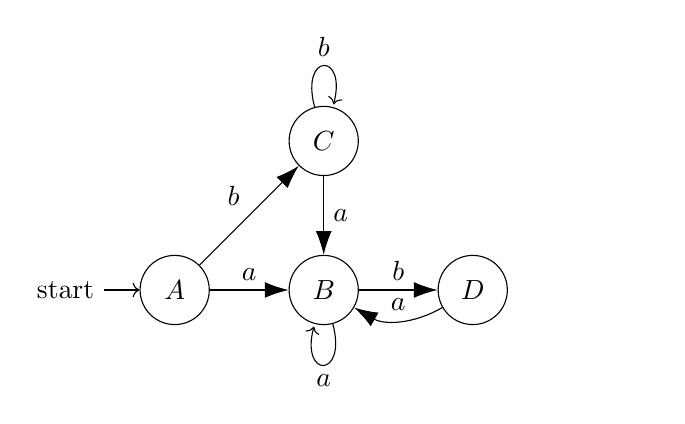
\begin{tikzpicture}[auto,
    ->,
    -{Latex[length=3mm,width=2mm]}
  ]
    \node[initial, state]   (A)                 {$A$};
    \node[state, draw=Black]            (B)  [right = of A] {$B$};
    \node[state, draw=Black]            (C)  [above = of B] {$C$};
    \node[state, draw=Black]            (D)  [right = of B] {$D$};
    \node[state, accepting, draw=none] (E)  [right = of D] {\ };
    
    \path (A) edge node {$a$} (B)
          (A) edge node {$b$} (C)
          (B) edge node {$b$} (D)
          (B) edge[loop below] node {$a$} (B)
          (C) edge node {$a$} (B)
          (C) edge[loop above] node {$b$} (C)
          (D) edge[bend left] node[above] {$a$} (B)
%          (D) edge node {$b$} (E)
%          (E) edge[bend left=40] node {$a$} (B)
%          (E) edge node[above] {$b$} (C)
    ;
    
  \end{tikzpicture}
}
\end{center}

\end{minipage}
\end{tabular}

\end{frame}
% frame end %%%%%%%%%%%%%%%%%%%%%%%%

% frame begin %%%%%%%%%%%%%%%%%%%%%%%%
\begin{frame}{NFA to DFA}
\myminorheader{Example}

\textbf{NFA:}

\begin{center}
\resizebox{0.5\textwidth}{!}{%
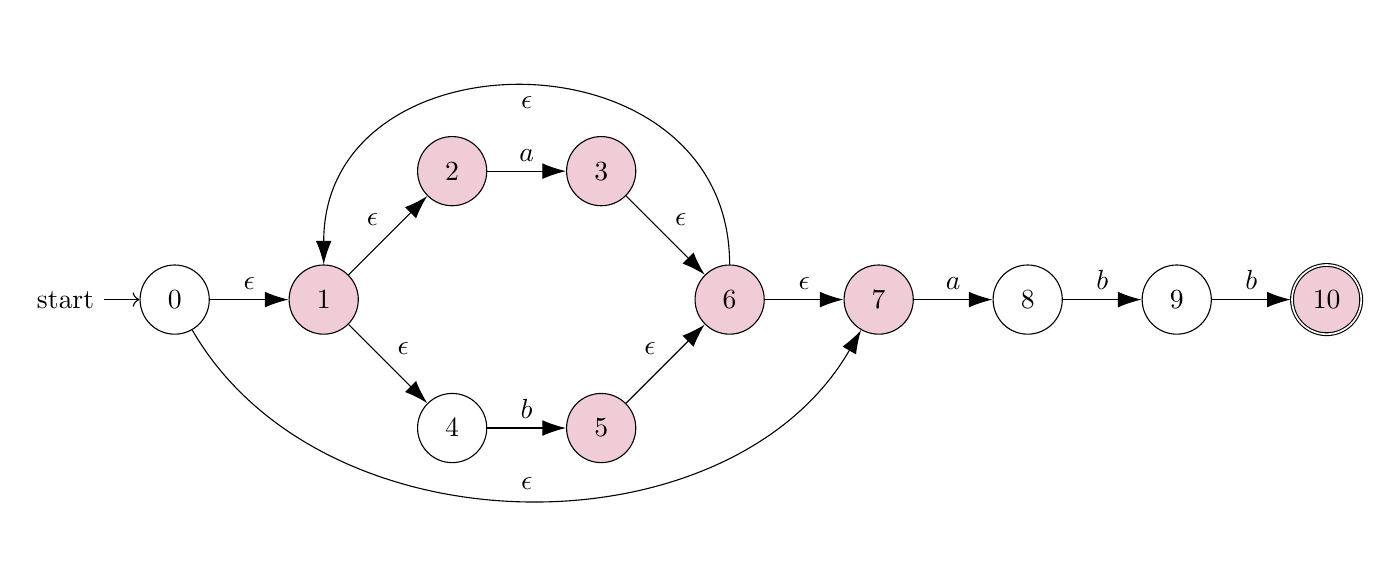
\begin{tikzpicture}[auto,
    ->,
    -{Latex[length=3mm,width=2mm]}
  ]
    \node[initial, state]   (0)                       {$0$};
    \node[state, fill=Pink!20]            (1)  [right = of 0]       {$1$};
    \node[state, fill=Pink!20]            (2)  [above right = of 1] {$2$};
    \node[state, fill=Pink!20]            (3)  [right = of 2]       {$3$};
    \node[state]            (4)  [below right = of 1] {$4$};
    \node[state, fill=Pink!20]            (5)  [right = of 4]       {$5$};
    \node[state, fill=Pink!20]            (6)  [below right = of 3] {$6$};
    \node[state, fill=Pink!20]            (7)  [right = of 6]       {$7$};
    \node[state]            (8)  [right = of 7]       {$8$};
    \node[state]            (9)  [right = of 8]       {$9$};
    \node[state, accepting, fill=Pink!20] (10) [right = of 9]       {$10$};
    
    \path (0) edge node {$\epsilon$} (1)
          (0) edge[bend right = 60] node {$\epsilon$} (7)
          (1) edge node {$\epsilon$} (2)
          (1) edge node {$\epsilon$} (4)
          (2) edge node {$a$} (3)
          (4) edge node {$b$} (5)
          (3) edge node {$\epsilon$} (6)
          (5) edge node {$\epsilon$} (6)
          (6) edge node {$\epsilon$} (7)
          (6.90) edge[bend right=90, min distance = 3 cm] node {$\epsilon$} (1.90)
          (7) edge node {$a$} (8)
          (8) edge node {$b$} (9)
          (9) edge node {$b$} (10)
          
          
    ;
    
  \end{tikzpicture}
}

{\scriptsize$DTrans(\{1,2,4,5,6,7,9\}, b) = \{1,2,3,5,6,7,10\}$}
\end{center}

\begin{tabular}{c @{\hspace{1cm}} c}
\begin{minipage}{0.3\textwidth}
\begin{tiny}
\begin{tabular}{|p{0.7\textwidth} | c | c |}
\hline
Subset & DFA & Marked \\
\hline
$\{0,1,2,4,7\}$       & $A$   & $\checkmark$ \\
\hline
$\{1,2,3,4,6,7,8\}$       & $B$   & $\checkmark$ \\
\hline
$\{1,2,4,5,6,7\}$       & $C$   & $\checkmark$ \\
\hline
$\{1,2,4,5,6,7,9\}$       & $D$   & $\checkmark$ \\
\hline
$\{1,2,3,5,6,7,10\}$       & $E$   & $\times$ \\
\hline
\end{tabular}
\end{tiny}
\end{minipage}
&
\begin{minipage}{0.7\textwidth}

\textbf{DFA:}
\begin{center}
\resizebox{0.6\textwidth}{!}{%
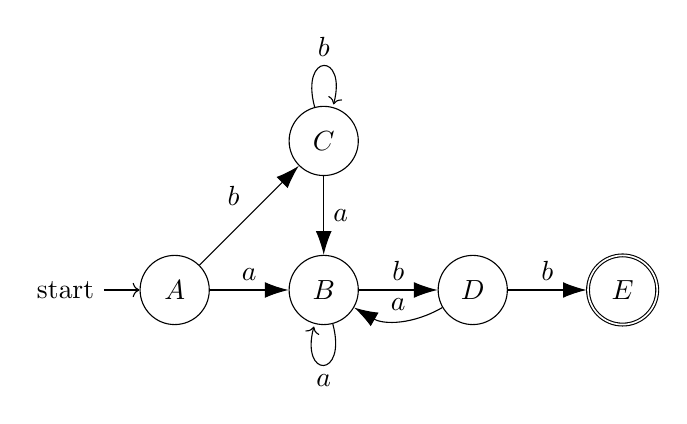
\begin{tikzpicture}[auto,
    ->,
    -{Latex[length=3mm,width=2mm]}
  ]
    \node[initial, state]   (A)                 {$A$};
    \node[state, draw=Black]            (B)  [right = of A] {$B$};
    \node[state, draw=Black]            (C)  [above = of B] {$C$};
    \node[state, draw=Black]            (D)  [right = of B] {$D$};
    \node[state, accepting, draw=Black] (E)  [right = of D] {$E$};
    
    \path (A) edge node {$a$} (B)
          (A) edge node {$b$} (C)
          (B) edge node {$b$} (D)
          (B) edge[loop below] node {$a$} (B)
          (C) edge node {$a$} (B)
          (C) edge[loop above] node {$b$} (C)
          (D) edge[bend left] node[above] {$a$} (B)
          (D) edge node {$b$} (E)
%          (E) edge[bend left=40] node {$a$} (B)
%          (E) edge node[above] {$b$} (C)
    ;
    
  \end{tikzpicture}
}
\end{center}

\end{minipage}
\end{tabular}

\end{frame}
% frame end %%%%%%%%%%%%%%%%%%%%%%%%

% frame begin %%%%%%%%%%%%%%%%%%%%%%%%
\begin{frame}{NFA to DFA}
\myminorheader{Example}

\textbf{NFA:}

\begin{center}
\resizebox{0.5\textwidth}{!}{%
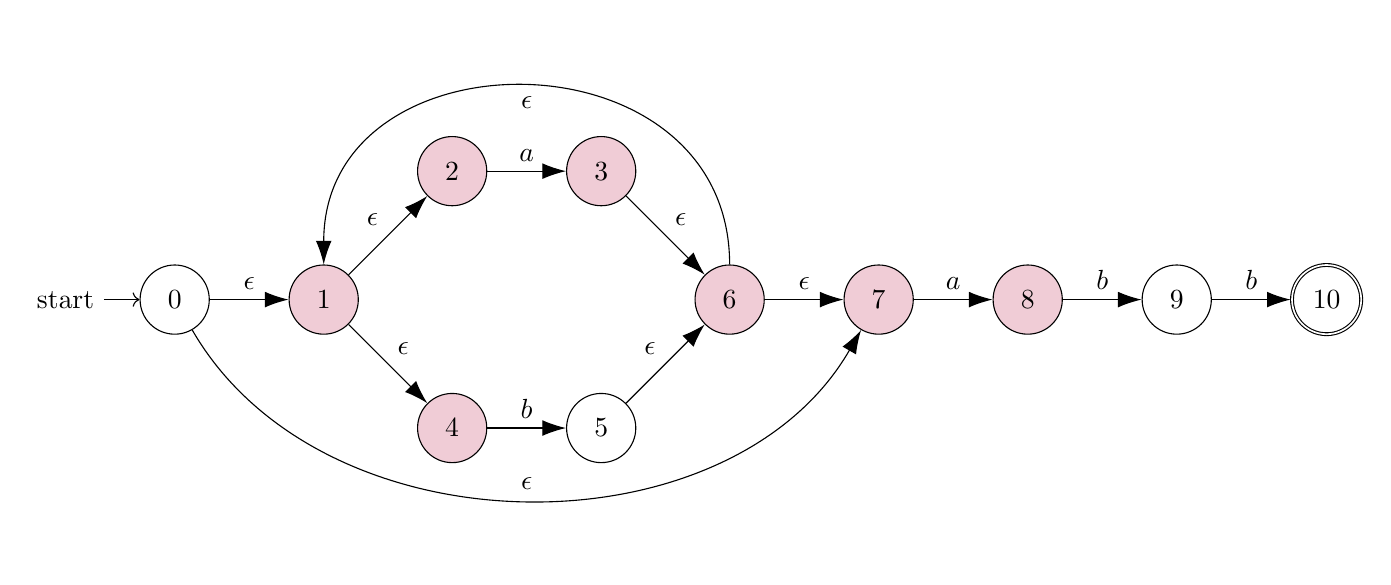
\begin{tikzpicture}[auto,
    ->,
    -{Latex[length=3mm,width=2mm]}
  ]
    \node[initial, state]   (0)                       {$0$};
    \node[state, fill=Pink!20]            (1)  [right = of 0]       {$1$};
    \node[state, fill=Pink!20]            (2)  [above right = of 1] {$2$};
    \node[state, fill=Pink!20]            (3)  [right = of 2]       {$3$};
    \node[state, fill=Pink!20]            (4)  [below right = of 1] {$4$};
    \node[state]            (5)  [right = of 4]       {$5$};
    \node[state, fill=Pink!20]            (6)  [below right = of 3] {$6$};
    \node[state, fill=Pink!20]            (7)  [right = of 6]       {$7$};
    \node[state, fill=Pink!20]            (8)  [right = of 7]       {$8$};
    \node[state]            (9)  [right = of 8]       {$9$};
    \node[state, accepting] (10) [right = of 9]       {$10$};
    
    \path (0) edge node {$\epsilon$} (1)
          (0) edge[bend right = 60] node {$\epsilon$} (7)
          (1) edge node {$\epsilon$} (2)
          (1) edge node {$\epsilon$} (4)
          (2) edge node {$a$} (3)
          (4) edge node {$b$} (5)
          (3) edge node {$\epsilon$} (6)
          (5) edge node {$\epsilon$} (6)
          (6) edge node {$\epsilon$} (7)
          (6.90) edge[bend right=90, min distance = 3 cm] node {$\epsilon$} (1.90)
          (7) edge node {$a$} (8)
          (8) edge node {$b$} (9)
          (9) edge node {$b$} (10)
          
          
    ;
    
  \end{tikzpicture}
}

{\scriptsize$DTrans(\{1,2,3,5,6,7,10\}, a) = \{1,2,3,4,6,7,8\}$}
\end{center}

\begin{tabular}{c @{\hspace{1cm}} c}
\begin{minipage}{0.3\textwidth}
\begin{tiny}
\begin{tabular}{|p{0.7\textwidth} | c | c |}
\hline
Subset & DFA & Marked \\
\hline
$\{0,1,2,4,7\}$       & $A$   & $\checkmark$ \\
\hline
$\{1,2,3,4,6,7,8\}$       & $B$   & $\checkmark$ \\
\hline
$\{1,2,4,5,6,7\}$       & $C$   & $\checkmark$ \\
\hline
$\{1,2,4,5,6,7,9\}$       & $D$   & $\checkmark$ \\
\hline
$\{1,2,3,5,6,7,10\}$       & $E$   & $\times$ \\
\hline
\end{tabular}
\end{tiny}
\end{minipage}
&
\begin{minipage}{0.7\textwidth}

\textbf{DFA:}
\begin{center}
\resizebox{0.6\textwidth}{!}{%
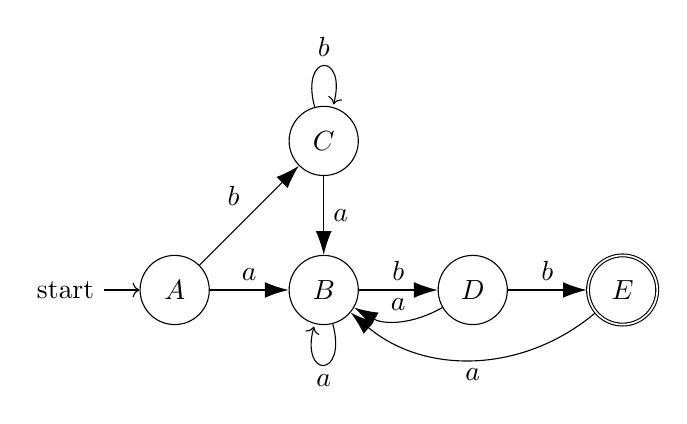
\begin{tikzpicture}[auto,
    ->,
    -{Latex[length=3mm,width=2mm]}
  ]
    \node[initial, state]   (A)                 {$A$};
    \node[state, draw=Black]            (B)  [right = of A] {$B$};
    \node[state, draw=Black]            (C)  [above = of B] {$C$};
    \node[state, draw=Black]            (D)  [right = of B] {$D$};
    \node[state, accepting, draw=Black] (E)  [right = of D] {$E$};
    
    \path (A) edge node {$a$} (B)
          (A) edge node {$b$} (C)
          (B) edge node {$b$} (D)
          (B) edge[loop below] node {$a$} (B)
          (C) edge node {$a$} (B)
          (C) edge[loop above] node {$b$} (C)
          (D) edge[bend left] node[above] {$a$} (B)
          (D) edge node {$b$} (E)
          (E) edge[bend left=40] node {$a$} (B)
%          (E) edge node[above] {$b$} (C)
    ;
    
  \end{tikzpicture}
}
\end{center}

\end{minipage}
\end{tabular}

\end{frame}
% frame end %%%%%%%%%%%%%%%%%%%%%%%%

% frame begin %%%%%%%%%%%%%%%%%%%%%%%%
\begin{frame}{NFA to DFA}
\myminorheader{Example}

\textbf{NFA:}

\begin{center}
\resizebox{0.5\textwidth}{!}{%
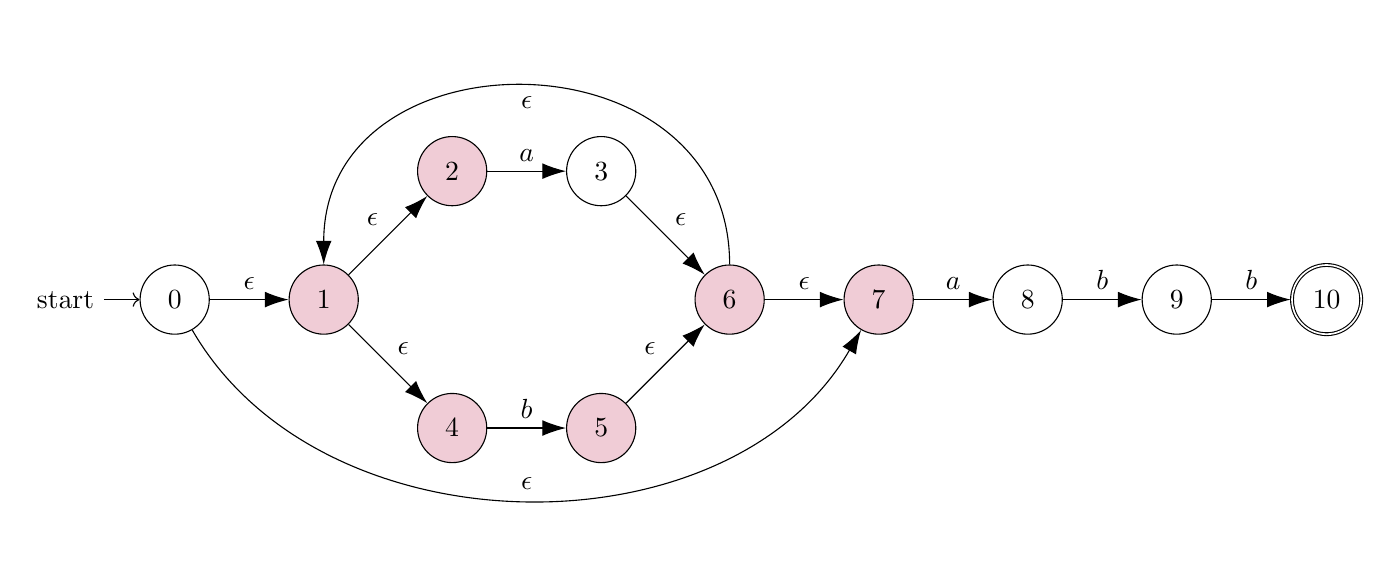
\begin{tikzpicture}[auto,
    ->,
    -{Latex[length=3mm,width=2mm]}
  ]
    \node[initial, state]   (0)                       {$0$};
    \node[state, fill=Pink!20]            (1)  [right = of 0]       {$1$};
    \node[state, fill=Pink!20]            (2)  [above right = of 1] {$2$};
    \node[state]            (3)  [right = of 2]       {$3$};
    \node[state, fill=Pink!20]            (4)  [below right = of 1] {$4$};
    \node[state, fill=Pink!20]            (5)  [right = of 4]       {$5$};
    \node[state, fill=Pink!20]            (6)  [below right = of 3] {$6$};
    \node[state, fill=Pink!20]            (7)  [right = of 6]       {$7$};
    \node[state]            (8)  [right = of 7]       {$8$};
    \node[state]            (9)  [right = of 8]       {$9$};
    \node[state, accepting] (10) [right = of 9]       {$10$};
    
    \path (0) edge node {$\epsilon$} (1)
          (0) edge[bend right = 60] node {$\epsilon$} (7)
          (1) edge node {$\epsilon$} (2)
          (1) edge node {$\epsilon$} (4)
          (2) edge node {$a$} (3)
          (4) edge node {$b$} (5)
          (3) edge node {$\epsilon$} (6)
          (5) edge node {$\epsilon$} (6)
          (6) edge node {$\epsilon$} (7)
          (6.90) edge[bend right=90, min distance = 3 cm] node {$\epsilon$} (1.90)
          (7) edge node {$a$} (8)
          (8) edge node {$b$} (9)
          (9) edge node {$b$} (10)
          
          
    ;
    
  \end{tikzpicture}
}

{\scriptsize$DTrans(\{1,2,3,5,6,7,10\}, b) = \{1,2,4,5,6,7\}$}
\end{center}

\begin{tabular}{c @{\hspace{1cm}} c}
\begin{minipage}{0.3\textwidth}
\begin{tiny}
\begin{tabular}{|p{0.7\textwidth} | c | c |}
\hline
Subset & DFA & Marked \\
\hline
$\{0,1,2,4,7\}$       & $A$   & $\checkmark$ \\
\hline
$\{1,2,3,4,6,7,8\}$       & $B$   & $\checkmark$ \\
\hline
$\{1,2,4,5,6,7\}$       & $C$   & $\checkmark$ \\
\hline
$\{1,2,4,5,6,7,9\}$       & $D$   & $\checkmark$ \\
\hline
$\{1,2,3,5,6,7,10\}$       & $E$   & $\checkmark$ \\
\hline
\end{tabular}
\end{tiny}
\end{minipage}
&
\begin{minipage}{0.7\textwidth}
\textbf{DFA:}
\begin{center}
\resizebox{0.6\textwidth}{!}{%
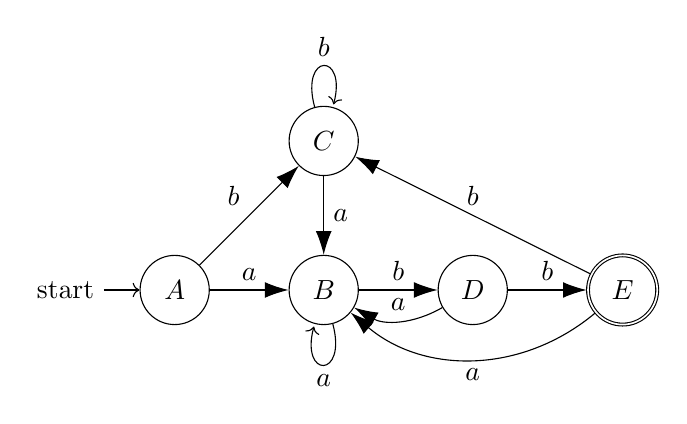
\begin{tikzpicture}[auto,
    ->,
    -{Latex[length=3mm,width=2mm]}
  ]
    \node[initial, state]   (A)                 {$A$};
    \node[state, draw=Black]            (B)  [right = of A] {$B$};
    \node[state, draw=Black]            (C)  [above = of B] {$C$};
    \node[state, draw=Black]            (D)  [right = of B] {$D$};
    \node[state, accepting, draw=Black] (E)  [right = of D] {$E$};
    
    \path (A) edge node {$a$} (B)
          (A) edge node {$b$} (C)
          (B) edge node {$b$} (D)
          (B) edge[loop below] node {$a$} (B)
          (C) edge node {$a$} (B)
          (C) edge[loop above] node {$b$} (C)
          (D) edge[bend left] node[above] {$a$} (B)
          (D) edge node {$b$} (E)
          (E) edge[bend left=40] node {$a$} (B)
          (E) edge node[above] {$b$} (C)
    ;
    
  \end{tikzpicture}
}
\end{center}

\end{minipage}
\end{tabular}


\end{frame}
% frame end %%%%%%%%%%%%%%%%%%%%%%%%


% frame begin %%%%%%%%%%%%%%%%%%%%%%%%
\begin{frame}{Next}

\pause
\myheader{Implementation of FSAs}
\end{frame}
% frame end %%%%%%%%%%%%%%%%%%%%%%%%

\end{document}
